\chapter{Aplikace}
Vzhledem ke komplexnosti aplikace je pro přehlednost rozdělena do několik složek.
\section{Prisma}

Databázové schéma v jazyku Prisma a databázové migrace se nachází ve složce \code{/prisma/}. Po úpravě Databázové schématu je dobré i vytvořit databázovou migraci, ta nám umožní manuálně spustit SQL příkazy, které Prisma vykonala pokud to bude potřeba.
Následuje vizualizace Databázové schématu vygenerovaná pomocí webové aplikace Prismaliser \cite{prismaliser}.
\begin{figure}[hbt!]
    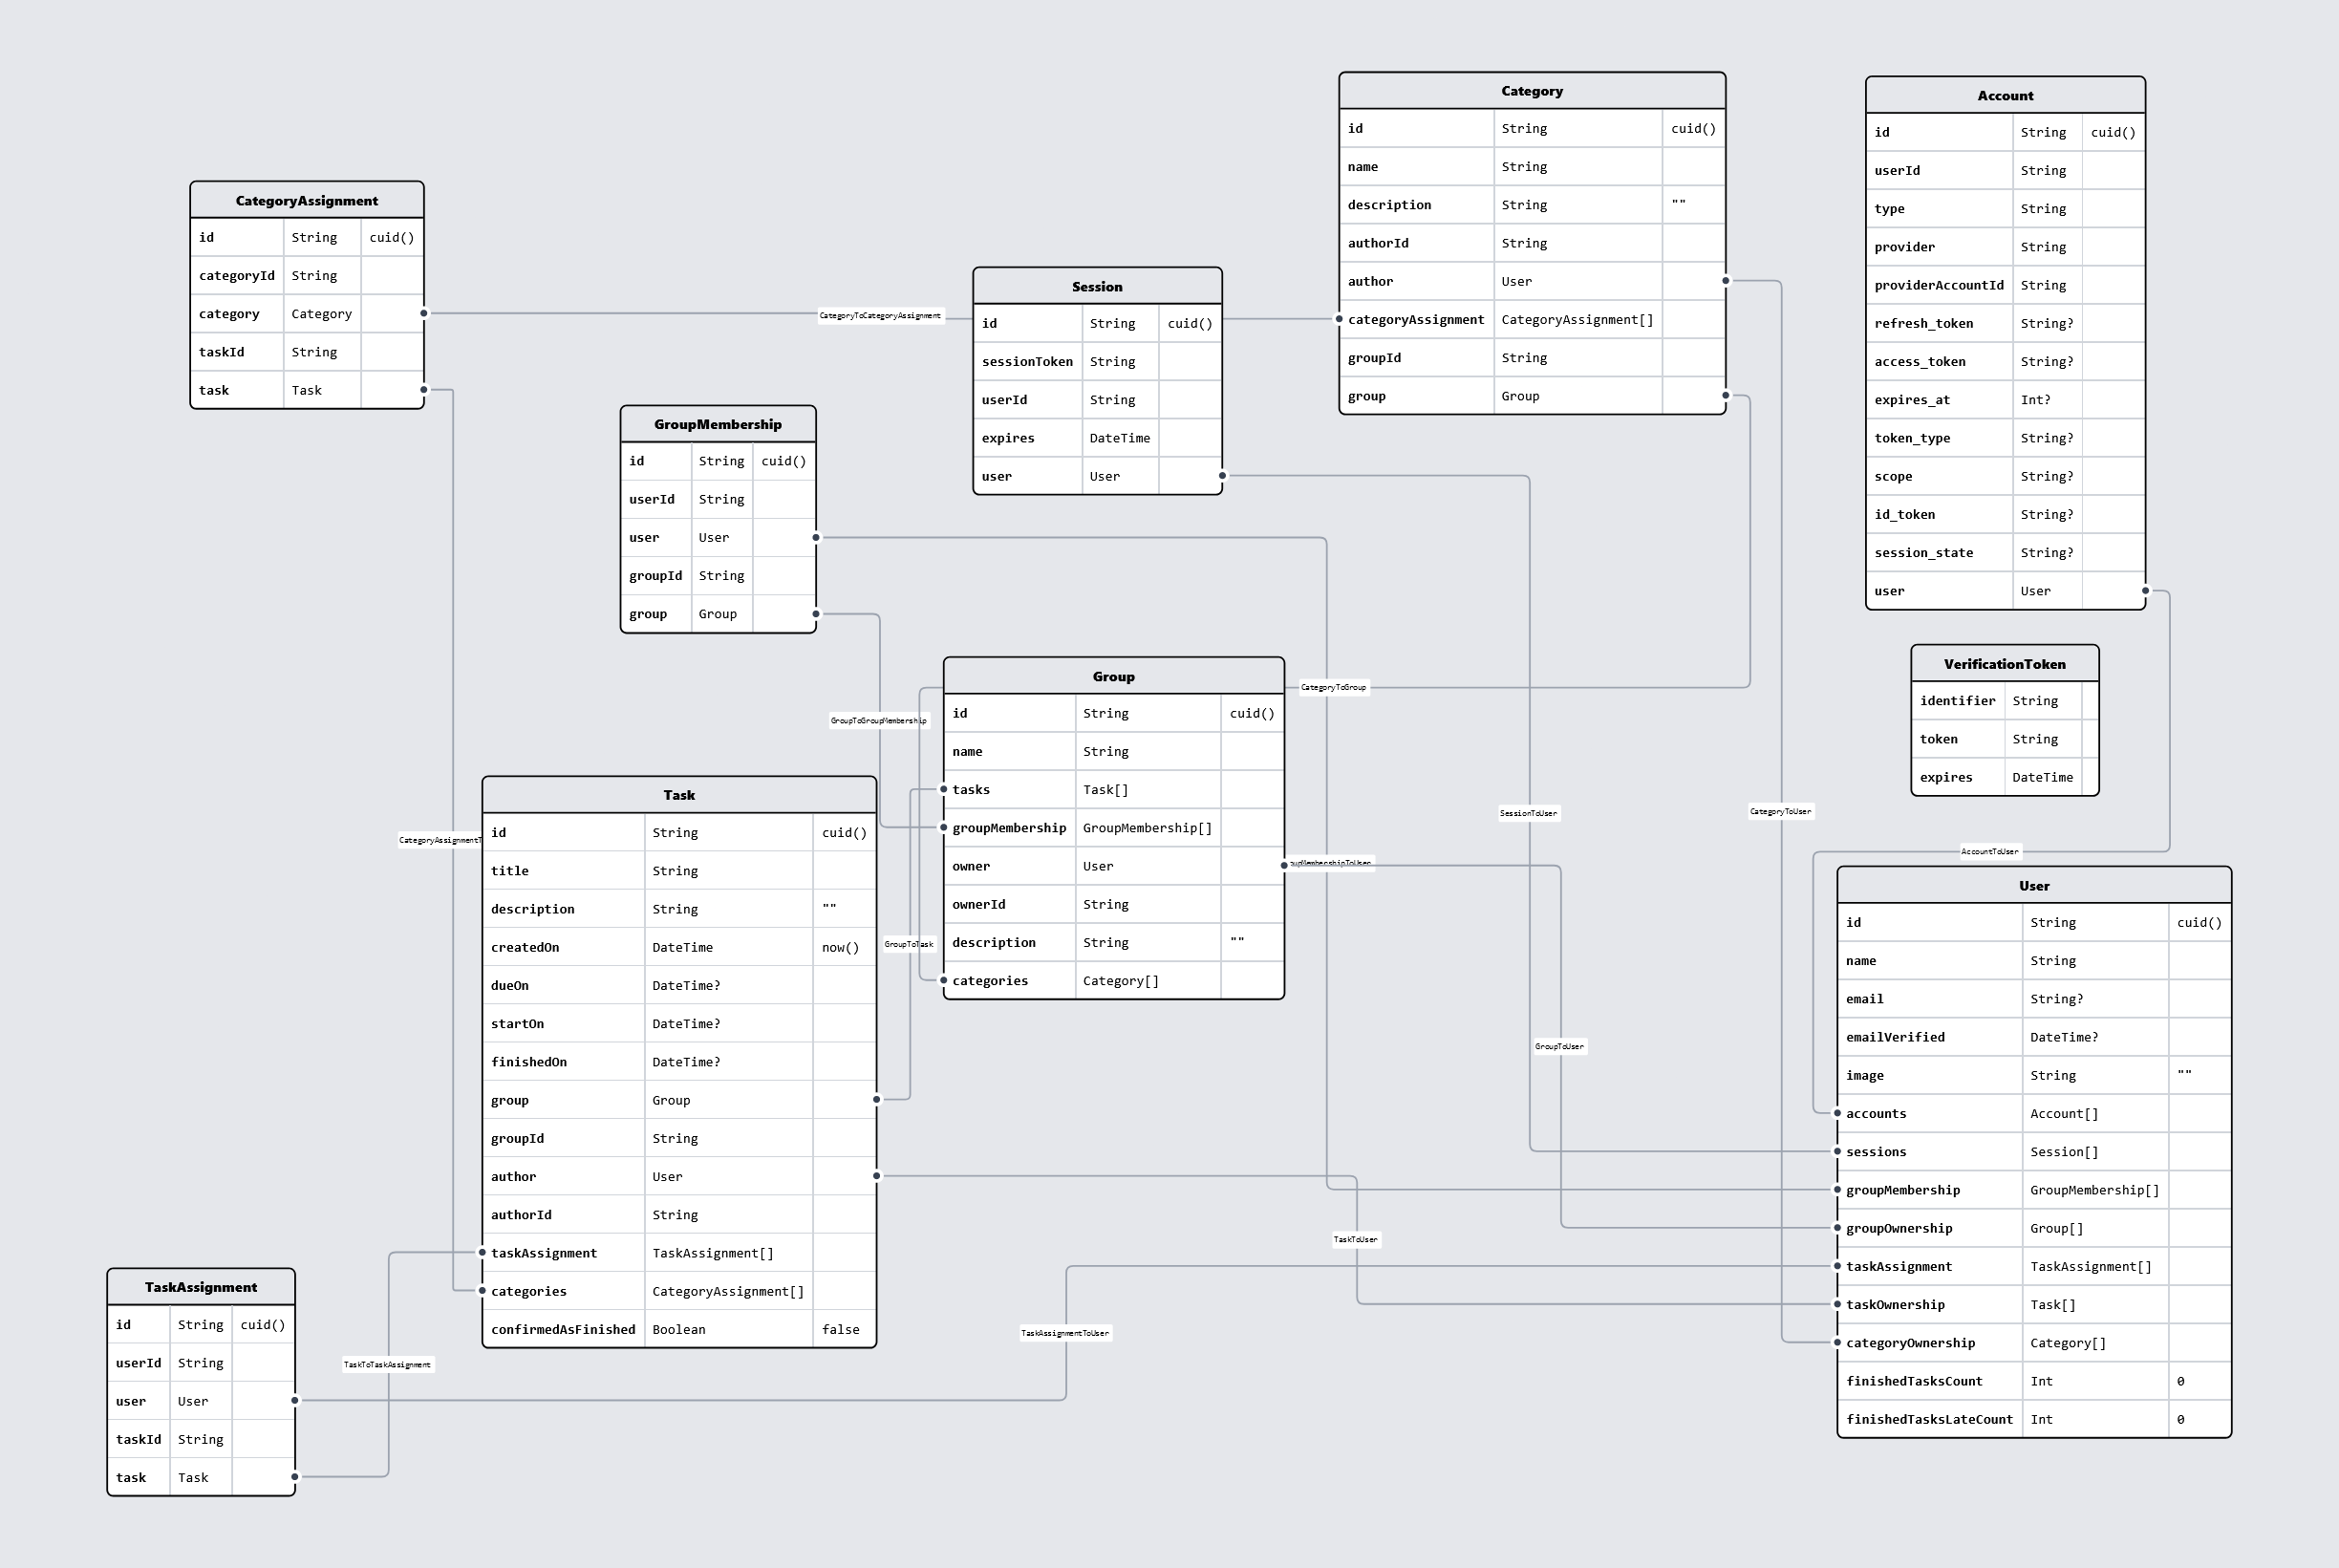
\includegraphics[width=1\linewidth]{img/DB_schema.png}
    \caption{Databázové schéma}
\end{figure}
\section{API}
Jak již zaznělo, celé API je psané za pomocí tRPC, to se nachází ve složce \code{/src/server/api/}.
API je inicializováno v souborech \code{trpc.ts} a \code{root.ts}. Konktrétně v souboru \code{trpc.ts} inicializujeme objekt tRPC a v \code{root.ts} na něj napojujeme jednotlivé Routery. Samotné "Endpointy", tedy přístupy, jsou rozděleny do "Routerů", ty se nachází ve složce \code{/src/server/api/routers} a dělí se na jednotlivé "hlavní objekty" v databázi. Tyto routery jsou děleny na soubory \code{categories.ts}, \code{groups.ts}, \code{tasks.ts} a \code{users.ts}. V kódu se "Endpointy" označují jako "Procedury", v princpu existují dva druhy procedur; Public\footnote{Veřejná} a Protected\footnote{Chráněná}. Jediným rozdílem mezi nimi je, že Protected procedura zaručuje, že jí může úspěšně zavolat pouze přihlášený uživatel.
Následuje úryvek z Routeru pro skupiny v souboru \code{groups.ts}. Ostatní procedury byly z ukázky odstraněny.
\begin{lstlisting}[caption={Procedura na přidání uživatele do skupiny}]
import { z } from "zod";

import {
  createTRPCRouter,
  protectedProcedure,
  publicProcedure,
} from "~/server/api/trpc";

export const groupsRouter = createTRPCRouter({
...
addMember: protectedProcedure
    .input(z.object({ userId: z.string(), groupId: z.string() }))
    .mutation(async ({ ctx, input }) => {
      const group = await ctx.prisma.group.findFirst({
        where: { id: input.groupId },
      });
      if (!group) throw new Error("Group not found");
      const user = await ctx.prisma.user.findFirst({
        where: { id: input.userId },
      });
      if (!user) throw new Error("User not found");
      if (group.ownerId !== ctx.session.user.id)
        throw new Error("You are not the owner of this group");
      const membership = await ctx.prisma.groupMembership.create({
        data: {
          groupId: input.groupId,
          userId: input.userId,
        },
      });
      if (membership) return true;
      return false;
    }),
...
})
\end{lstlisting}
Jako první musíme definovat název Procedury, v tomto případě "addMember", tedy "přidatUživatele". Dále přidáme \code{.input()} zde bude přijímat procedura data pro své provedení. Pokud bude Procedura data měnit tak přidáme \code{.mutation}, pokud data pouze předá z Databáze tak přidáme \code{.query}. Do těch poté předáme vstup z \code{.input} a \code{ctx}\footnote{Kontext}. Kontext je globálně zpracovávaný a nachází se v něm \code{session} přihlášeného uživatele a \code{prisma}, tou se napojujeme na databázi.
\subsection{Příklad API Endpointů}
    \begin{tabularx}{1\textwidth} { 
  | >{\centering\arraybackslash}X 
  | >{\centering\arraybackslash}X 
  | >{\centering\arraybackslash}X 
  | >{\centering\arraybackslash}X 
  | >{\centering\arraybackslash}X | }
     \hline
        \textbf{Router} & \textbf{Název} & \textbf{Popis} & \textbf{Vstup} & \textbf{Výstup}\\
         \hline
         tasks.ts & assignUser & Přiřadí uživatele k úkolu & ID uživatele, ID úkolu & True / False\\
          \hline
         tasks.ts & getCategories & Vrátí pole kategorií úkolu & ID úkolu & Category[]\\
         \hline
         groups.ts & getById & Vrátí objekt skupiny pokud je přihlášený uživatel člen & ID skupiny & Group\\
         \hline
         groups.ts & leave & Odstraní přihlášeného uživatele ze skupiny & ID skupiny & True / False\\
         \hline
         users.ts & locateByName & Vrátí pole uživatelů s podobným jménem k vstupu & Text & User[]\\
         \hline
         users.ts & editName & Upraví jméno uživatele & ID uživatele, Nové jmnéno & User\\
         \hline
         categories.ts & create & Vytvoří kategorii & Název, Popis, ID autora, ID skupiny & Category\\
         \hline
         categories.ts & getTasks & Vrátí úkoly s kategorií & ID kategorie & Task[]\\
         \hline
    \end{tabularx}